%%%%%%%%%%%%%%%%%%%%%%%%%%%%%%%%%%%%%%%%%%%%%%%%%%%%%%%%%%%%%%%%%%
\begin{frame}{Audio classification / segmentation}
  \framesubtitle{\cite{Jang19Music}}
  \begin{center}
    \includegraphics[width=0.6\textwidth]{../figs/music_speech}    
  \end{center}
  \begin{itemize}
  \item Classification at each time step
  \item But the context is crucial (for the input and the output) ! 
  \item \important{Spectrogram ?}
  \end{itemize}
\end{frame}


%%%%%%%%%%%%%%%%%%%%%%%%%%%%%%%%%%%%%%%%%%%%%%%%%%%%%%%%%%%%%%%%%%
\begin{frame}{Interlude: the input spectrogram}
  \begin{center}
    \includegraphics[width=0.5\textwidth]{../figs/speech_1}\\
    $\downarrow$ \\
    Segmentation in frames (Hamming window)\\
    $\downarrow$ \\
    F.F.T \\
    $\downarrow$ \\
    Mel Filters \\
    $\downarrow$ \\
    Log\\
    $\downarrow$ \\
    D.C.T  \\
    $\downarrow$ \\
    \includegraphics[width=0.5\textwidth]{../figs/speech_2}\\
  \end{center}
\end{frame}



\begin{frame}{Human activity Recognition}
  \begin{block}{The data}
    10k samples of fixed length (128 points at 50kHz)
    \footnote{\url{https://archive.ics.uci.edu/ml/datasets/human+activity+recognition+using+smartphones}}:
    \begin{itemize}
    \item x, y, and z accelerometer data (linear acceleration) 
    \item and the three gyroscopic data (angular velocity)
    \end{itemize}
    The classes are: Walking, Upstairs,  Downstairs,  Sitting,  Standing, Laying. 
  \end{block}
  \begin{itemize}
  \item[$\rightarrow$] Two different input channels (accelerometer and
    gyroscopic).
  \item[$\rightarrow$] How to define a convolution filter for two
    input channels ?
  \item[$\rightarrow$] The sequence is long but of fixed size, the
    overall max-pooling is maybe not the best option.
  \end{itemize}
\end{frame}


\begin{frame}{Convolution 1D with 2 input channels}
    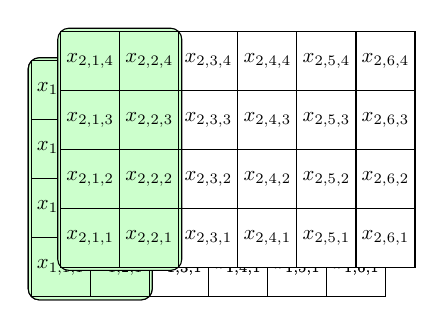
\begin{tikzpicture}[scale=0.75,every node/.style={scale=0.75}]
      % the window 
      % offset for x and y of .5 + a bit more
      %%%% channel 1 
      \draw[fill=green!20,rounded corners] (0.45,0.45) rectangle (2.55,4.55); % green 
      %% the grid 
      \foreach \l in {1,2,...,4}
      \foreach \c in {1,2,...,6}
      {
        \draw (\c,\l) +(-.5,-.5) rectangle ++(.5,.5);
        \draw (\c,\l) node{$x_{1,\c,\l}$};
      }
      %%%% channel 1 
      \draw[fill=green!20,rounded corners] (0.45,0.45) rectangle (2.55,4.55); % green 
      %% the grid 
      \foreach \l in {1,2,...,4}
      \foreach \c in {1,2,...,6}
      {
        \draw (\c,\l) +(-.5,-.5) rectangle ++(.5,.5);
        \draw (\c,\l) node{$x_{1,\c,\l}$};
      }
      %\pause
      %%%% channel 2 
      \draw[fill=white] (1,1) rectangle (7,5);
      \draw[fill=green!20,rounded corners] (0.95,0.95) rectangle (3.05,5.05); % green 
      %% the grid 
      \foreach \l in {1,2,...,4}
      \foreach \c in {1,2,...,6}
      {
        \draw (\c,\l) rectangle ++(1,1);
        \draw (\c,\l)+(0.5,0.5) node{$x_{2,\c,\l}$};
      }
    \end{tikzpicture}
    \hfill
    %\pause
    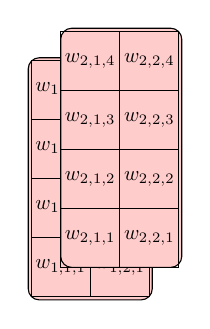
\begin{tikzpicture}[scale=0.75,every node/.style={scale=0.75}]
      %%% channel 1 
      % the window
      % offset for x and y of .5 + a bit more 
      \draw[fill=red!20,rounded corners] (0.45,0.45) rectangle (2.55,4.55); % green 
      %% the grid 
      \foreach \l in {1,2,...,4}
      \foreach \c in {1,2}
      {
        \draw (\c,\l) +(-.5,-.5) rectangle ++(.5,.5);
        \draw (\c,\l) node{$w_{1,\c,\l}$};
      }
      %\pause
      %%% channel 2
      \draw[fill=red!20,rounded corners] (1,1) rectangle (3.05,5.05); % green 
      %% the grid 
      \foreach \l in {1,2,...,4}
      \foreach \c in {1,2}
      {
        \draw (\c,\l) rectangle ++(1,1);
        \draw (\c,\l)+(0.5,0.5) node{$w_{2,\c,\l}$};
      }
    \end{tikzpicture}
    \begin{block}{The output value (output channel)}
      $$
      \textrm{At time }t = 1,\ {\color{red!70!black} h_1} = \sum_{k,i,j} {\color{red!70!black}w_{k,i,j}}\times  {\color{green!70!black}x_{k,i,j}}
      $$
    \end{block}
    We can have multiple input and output channels. 
  \end{frame}



  \begin{frame}{Convolution 1D and max-pooling in pytorch}
    \begin{columns}
      \column{0.5\textwidth}
      \begin{block}{Convolution 1D}
        torch.nn.Conv1d(
        \begin{itemize}
        \item in\_channels, 
        \item out\_channels, 
        \item kernel\_size, 
        \item stride=1, 
        \item padding=0,
        \item dilation=1, ...
        \end{itemize}
        )
      \end{block}
      \column{0.5\textwidth}
      \begin{block}{Max-Pooling 1D}
      torch.nn.MaxPool1d(
      \begin{itemize}
      \item kernel\_size, 
      \item stride=None, 
      \item padding=0, 
      \item dilation=1,
      \item return\_indices=False, 
      \item ceil\_mode=False
      \end{itemize}
      )
    \end{block}
    \end{columns}
  \end{frame}




